\documentclass[tikz,border=4pt]{standalone}
\usepackage{amsmath,amssymb}
\usetikzlibrary{positioning,arrows.meta,calc,fit}
\begin{document}
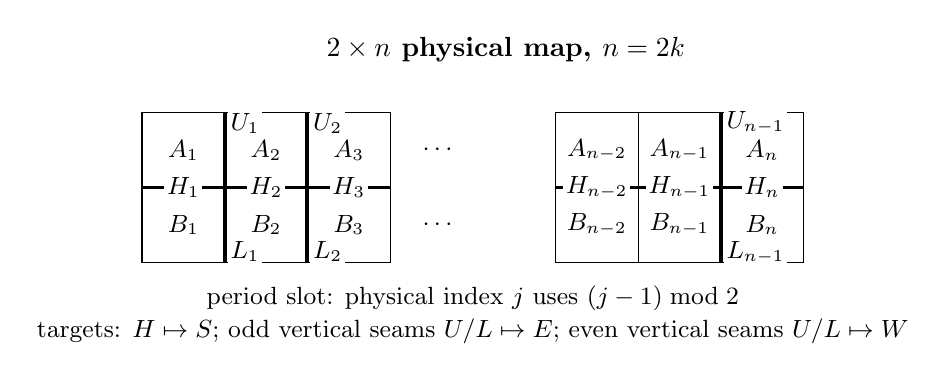
\begin{tikzpicture}[x=1.05cm,y=0.95cm,font=\small,>=Latex]
\node[font=\bfseries] at (4.4,2.85) {$2\times n$ physical map, $n=2k$};

% First three contiguous columns.
\foreach \x/\lab in {0/1,1/2,2/3}{
  \draw (\x,1) rectangle +(1,1);
  \draw (\x,0) rectangle +(1,1);
  \node at (\x+.5,1.5) {$A_{\lab}$};
  \node at (\x+.5,.5) {$B_{\lab}$};
  \draw[line width=1.2pt] (\x,1)--(\x+1,1);
  \node[fill=white,inner sep=1pt] at (\x+.5,1) {$H_{\lab}$};
}
% Ellipsis gap.
\node at (3.6,1.5) {$\cdots$};
\node at (3.6,.5) {$\cdots$};
% Final three contiguous columns.
\foreach \x/\lab in {5/{n-2},6/{n-1},7/n}{
  \draw (\x,1) rectangle +(1,1);
  \draw (\x,0) rectangle +(1,1);
  \node at (\x+.5,1.5) {$A_{\lab}$};
  \node at (\x+.5,.5) {$B_{\lab}$};
  \draw[line width=1.2pt] (\x,1)--(\x+1,1);
  \node[fill=white,inner sep=1pt] at (\x+.5,1) {$H_{\lab}$};
}

% Physical vertical seams, drawn directly on shared face boundaries.
\foreach \x/\lab in {1/1,2/2,7/{n-1}}{
  \draw[line width=1.5pt] (\x,1)--(\x,2);
  \draw[line width=1.5pt] (\x,0)--(\x,1);
  \node[fill=white,inner sep=1pt,anchor=south west] at (\x+.03,1.68) {$U_{\lab}$};
  \node[fill=white,inner sep=1pt,anchor=north west] at (\x+.03,.32) {$L_{\lab}$};
}

\node[align=center] at (4,-.48) {period slot: physical index $j$ uses $(j-1)\bmod 2$};
\node[align=center] at (4,-.92) {targets: $H\mapsto S$; odd vertical seams $U/L\mapsto E$; even vertical seams $U/L\mapsto W$};
\end{tikzpicture}
\end{document}
